%!TEX root = ../thesis.tex

% Definitions:
%%%%%%%%%%%%%%
% Semantiv Web = samantisches Web

\chapter{Grundlagen} % (fold)
\label{cha:grundlagen}

\section{Semantic Web} % (fold)
\label{sec:semantic_web}

% section semantic_web (end)

\subsection{Resource Description Framework} % (fold)
\label{sub:resource_description_language}

Eine der bekanntesten Umsetzungen der Vision des  semantischen Webs ist wohl das Resource Description Framework (RDF). Wie der Name schon suggeriert dient RDF zur Beschreibung von einzelnen Ressourcen innerhalb des Internets. Nach \cite{Klyne2004,Manola2004} bestand die Motivation bei der Entwicklung von RDF Information über Ressource in einen offenen Datenmodell zu speichern, so dass diese Daten von Maschinen automatisch verarbeitet, manipulieren und untereinander ausgetauscht werden können. Gleichzeitig sollte es auch einfach von jedem erweitert werden können \enquote{RDF is designed to represent information in a minimally constraining, flexible way}\cite{Klyne2004}.

\medskip

Das Datenmodell von RDF ist sehr einfach aufgebaut um es effizient verarbeiten zu können. Die Grundlage bilden simple Tripel aus Subjekt, Prädikat und Objekt, welche an die natürliche Sprache angelehnt als Sätze\cite{Heinzen} bezeichnet werden. Mehrere solcher Tripel bilden einen RDF Graphen. Das Prädikat beschreibt hierbei eine Beziehung zwischen Subjekt und Objekt und wird daher oft als Eigenschaft beschrieben. In der natürlichen Sprache kann man dies zum Beispiel so ausdrücken; Das Subjekt hat eine Eigenschaft mit den Wert Objekt. Graphisch wird dies durch eine gerichtete Verbindung von Subjekt und Objekt mit der Beschriftung der Prädikats dargestellt (siehe Abbildung \ref{fig:graphische_darstellung_eines_rdf_tripels}).

\medskip

\begin{figure}[h]
    \centering
    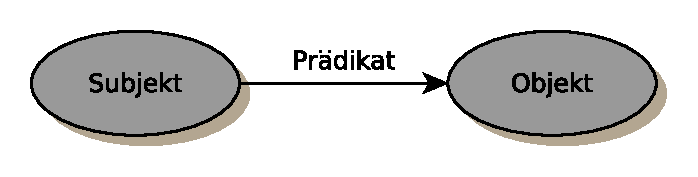
\includegraphics[scale=0.7]{assets/images/rdf-triple}
    \caption{Graphische Darstellung eines RDF Tripels}
    \label{fig:graphische_darstellung_eines_rdf_tripels}
\end{figure} 

Für Subjekt, Prädikat und Objekt besteht die Möglichkeit sogenannte Uniform Resource Identifiers (URI), Literale oder leere Knoten als Werte einzusetzen. 

\begin{description}
    \item[URIs] sind eindeutige Bezeichner die eine beliebige reale oder abstrakte Ressource und werden wie in RFC 2396\footnote{\url{http://www.isi.edu/in-notes/rfc2396.txt}} beschrieben formatiert, wobei relative URIs nach \cite{Klyne2004} nicht verwendete werden sollen.
    \item[Literale] bestehen aus einfachen Zeichenketten die zum Speichern der Informationen dienen. Zusätzlich können Literale mit der Angabe der verwendeten Sprache \lstinline[basicstyle=\ttfamily]{"Objekt"@de} oder des Datentyps \lstinline[basicstyle=\ttfamily]{"42"^^xsd:integer} erweitert werden. Bei Literalen ist aber auch darauf zu achten, dass \lstinline[basicstyle=\ttfamily]{"Objekt} und \lstinline[basicstyle=\ttfamily]{"Objekt"@de} beschreiben zwar beide den gleichen Wert werden aber von RDF nicht als gleich angesehen. Zwei Literale können nur gleich sein, wenn sie die selbe Sprache beziehungsweise den selben Datentyp besitzen.  
    \item[Leere Knoten] werden als alle Knoten im RDF Graphen beschrieben, welche weder eine URI noch ein Literal sind. Sie dienen häufig dazu um Subjekte zu beschreiben für die aber nicht unbedingt eine eigene URI nötig ist und sind nur innerhalb eines Graphen eindeutig \todo[inline]{Beispiel}.
\end{description}

Doch nicht jeder davon ist in jeden Teil des Tripels erlaubt. Das Subjekt ist entweder eine URI oder ein leerer Knoten wobei das Prädikat nur eine URI sein kann. Dahingegen ist es beim Objekt möglich eine URI, einen leeren Knoten oder ein Literal zu verwendeten. 

\subsubsection{RDF/XML, N3} % (fold)
\label{ssub:rdf_xml_n3}

\begin{description}
    \item[RDF/XML] 
    \item[N3] ist die Kurzform für Notation 3 und wurde von Tim Berners-Lee als Sprache für RDF entwickelt. Tripel in N3 werden dabei wie Sätze in meisten natürlichen Sprachen geschrieben. Erst das Subjekt, dann das Prädikat und am Ende das Objekt gefolgt von einen Punkt, wie in  Listing \ref{lst:n3_beispiel} zu sehen ist.
    \begin{lstlisting}[caption={Einfaches N3 Beispiel}\label{lst:n3_beispiel},captionpos=t]
<http://example.de/florian> <http://example.org/#name> "Florian" .
<http://example.de/florian> <http://example.org/#age> "28" .    \end{lstlisting} 
    Die URI \texttt{http://example.de/florian} beschreibt hierbei eine Ressource welche einen Namen \texttt{Florian} und ein Alter \texttt{28} besitzt. Es ist darauf zu achten, dass alle URI immer zwischen spitzen Klammern stehen. Da nun einzelne Prädikate recht häufig innerhalb eines Graphen auftauchen können, kann es einfach sein diese abgekürzt schreiben zu können. Hierzu ist es möglich sogenannte Präfixe (auch Namensräume genannt) am Beginn des Dokumentes zu definieren und einen so Schreibarbeit abzunehmen.

    \begin{lstlisting}[caption={Präfixe}\label{lst:n3_prefix},captionpos=t]
@prefix person: <http://example.org/#> .
<http://example.de/florian> person:name "Florian" .
<http://example.de/florian> person:age "28" .    \end{lstlisting}

    Am Anfang von Listing \ref{lst:n3_prefix} wird durch Einleiten mittels des Schlüsselwortes \texttt{@prefix} ein neuer Präfix \texttt{person:} für die URI \texttt{http://example.org/\#} festgelegt (man beachte wieder den Punkt am Ende der Zeile). Dieser Präfix kann nun überall innerhalb des Dokumentes verwendet werden, wobei die spitzen Klammern der vorherigen URI weggelassen werden können.

    \todo[inline]{Leere Knoten + kurz Turtle}

\end{description}

% subsubsection rdf_xml_n3_turtle (end)

\subsection{Abfragesprache SPARQL} % (fold)
\label{ssub:abfragesprache_sparql}

% subsubsection resource_description_language (end)

\subsection{Ontologien} % (fold)
\label{sub:ontologien}

% subsection ontologien (end)

% chapter grundlagen (end)
